\documentclass[12pt, a4]{article}
\usepackage{blindtext}
\usepackage{graphicx}
\usepackage{subcaption}
\usepackage{hyperref}
\usepackage{float}
\usepackage{amsmath}
\usepackage{amssymb}

\usepackage[margin=0.75in]{geometry}
\graphicspath{{./images/}}

\title{%
Finding the best position of centre of mass of cyclist and bike for most efficient safe braking \\
\large International Baccalureate Extended Essay}
\author{Igor Krzywda}

\begin{document}
\maketitle

\section{Introduction}\label{intro}
\subsection{Context}\label{intro_context}
Braking is the most important safety feature on a bicycle, however, when misused, braking can be the cause of the
most severe crashes one can have on a bicycle. Many of such crashes are caused by the lack of understanding of
mechanics of braking a bicycle. There are countless tutorials on how to brake properly on a bicycle, but most of
them are based on empirical experience of more proffesional riders [See Appendix A]. Such advice falls in line with physical 
analysis, but is mostly biased by many factors spanning from the type of cycling the tutorial is based on to 
the attitude towards crashing of the presenter. There is clearly a void in giving an objective advice on safety 
on a bicycle that can be a base to domain-specific guides.
\subsection{The goal of the research}\label{intro_goal_of_research}
The goal of the research is to create an universal model for finding the best braking position in terms of
centre of mass on any bicycle. Such model will serve as a basis for explaining why it is important to find 
a bike fitting its rider and giving the reader an idea of where the limits of his equipment are without 
finding about it by crashing.

\section{Theoretical analysis of braking a bicycle}\label{theory}
\subsection{Rules and assumptions for the analysis}\label{theory_rules}
Assumptions about bicycle and rider:
\begin{itemize}
\item{rider and bicycle make one rigid body}
\item{there is no dissipation of force}
\end{itemize}
Safe braking in the analysis is defined by two factors:
\begin{itemize}
\item{rear wheel makes contact with the surface at all times}
\item{no wheel is skidding while braking}
\end{itemize}
Neglected factors:
\begin{itemize}
\item{decrease in braking power due to heat and brake pad residue}
\item{dynamic change in frame geometry due to amortisation and tire compression}
\item{air drag}
\item{rolling resistance}
\end{itemize}
\subsection{Theoretical model of bicycle and cyclist}\label{theory_model}
The model of bike and a rider for this analysis is two dimensional, because no lateral forces are taken in 
consideration. The cases for safe braking are checked with the state of wheels, hence the focal point of the 
analysis will be forces excerted on axles, so the whole frame of the bike can be reduced to a single beam 
spanning from axle to axle. The rider is reduced to net centre of mass of bike and cyclist, which is connected
perpendicularly to the virtual beam. Figure~\ref{fig:theoretical_models} shows the simplification of the model.
\begin{figure}[H]
\caption{}
\centering
\begin{subfigure}[b]{0.3\linewidth}
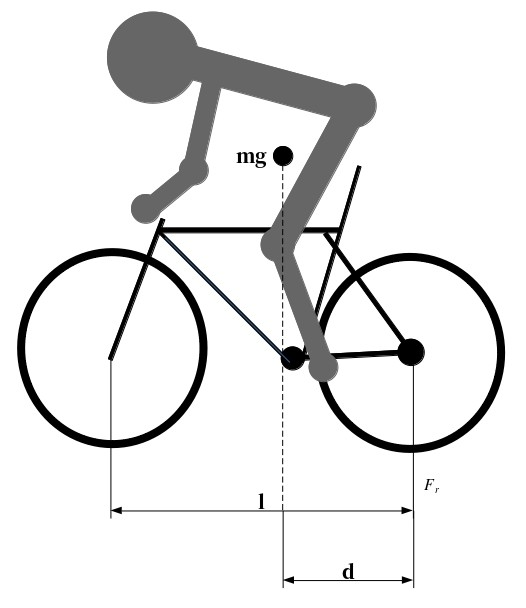
\includegraphics[width=\linewidth]{bike_static_model_bike}%
\label{fig:bike_diagram}
\caption{}
\end{subfigure}
\begin{subfigure}[b]{0.3\linewidth}
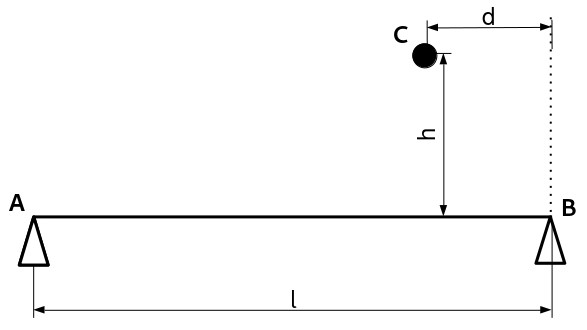
\includegraphics[width=\linewidth]{bike_static_model_simplified}
\caption{}%
\label{fig:beam_diagram}
\end{subfigure}%
\label{fig:theoretical_models}
\end{figure}
\subsection{Force distribution on the axles}\label{theory_force_distro}
The force distribution on the axles is the most important part of the analysis, as it gives us data to 
determine the deceleration and whether or not the conditions for safe braking are maintained.
\subsubsection{Cyclist static or moving at constant speed}\label{theory_force_distro_static}
\begin{figure}[H]
\centering
\caption{}
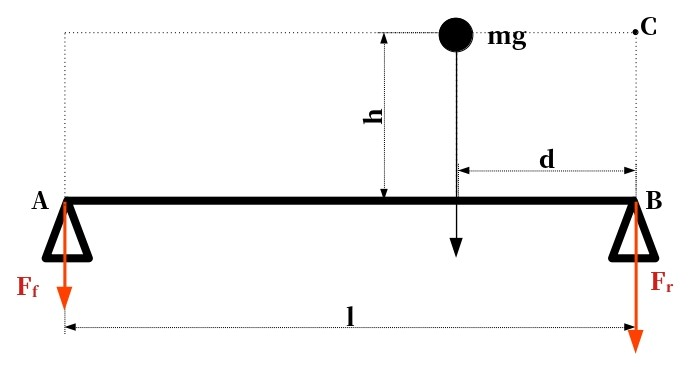
\includegraphics[width=0.5\linewidth]{static_forces_simplified}%
\label{fig:static_diagram}
\end{figure}
First let us consider the case of the cyclist being stationary or moving at a constant speed. In order to 
calculate the forces on each axle, we need to consider moments of force applied to the frame, which will be
our moment arm $l$ (fig.~\ref{fig:static_diagram}). When a cyclist is on the bike, the point on the frame, where
the force is being excerted is right below his centre of mass. In order to calculate the either of the forces 
on the axles, we need to equate internal torques to either point A or B in fig.~\ref{fig:static_diagram}: 
\begin{equation}
\centering%
\label{eq:equating_torques}
F_f \cdot l = mg \cdot d
\end{equation}
\begin{equation}
\centering%
\label{eq:F_f}
F_f(d) = \frac{mg \cdot d}{l}
\end{equation}
\begin{equation}
\centering%
\label{eq:F_r}
F_r(d) = mg - F_f(d)
\end{equation}
From this equation we can derive load on front axle~\eqref{eq:F_f}. The net reaction acting 
on the bike's axles is $mg$, therefore the load on rear axle will be described as in~\eqref{eq:F_r}
\begin{figure}[H]
\centering
\caption{\textit{Reaction on axles in relation to distance of centre of mass from the rear axle when stationary or at constant speed}}
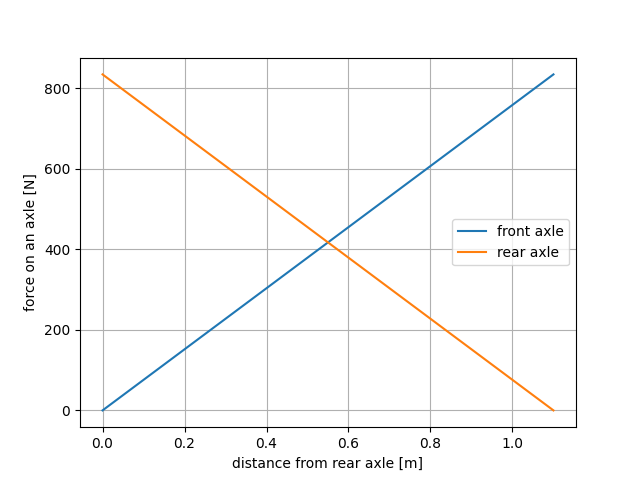
\includegraphics[width=0.5\linewidth]{axles_static_graph}%
\label{fig:static_graph}
\end{figure}
When we plot these functions, (fig.~\ref{fig:static_graph})\footnote[1]{See Appendix A for data used to generate the graphs}. 
The load on the front axle is a linear function with coefficient of $\frac{mg}{l}$, which means that the heavier the 
rider and bike, the steeper the graph. Same effect would have been making the bike shorter. The force on the rear 
axle is the inverse of front one.
\subsubsection{Cyclist decelerating}\label{theory_force_distro_dynamic}
\begin{figure}[H]
\centering
\caption{}
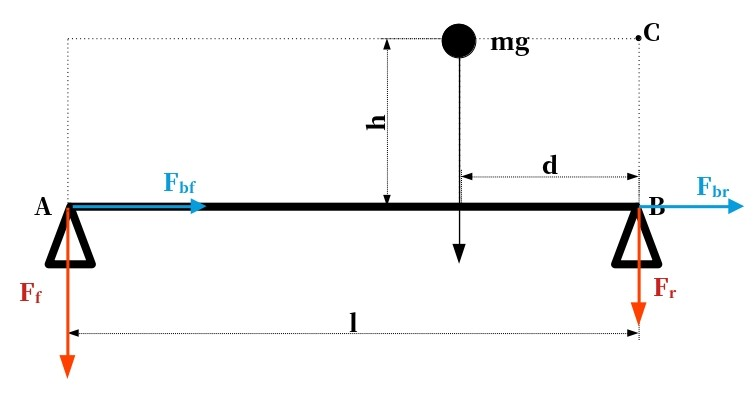
\includegraphics[width=0.5\linewidth]{decelerating_forces_diagram}%
\label{fig:deceleration_diagram}
\end{figure}
\begin{equation}
\centering%
\label{eq:eq_torques_dyn}
F_f \cdot l = mg \cdot d + (F_{bf} + F_{br}) \cdot h
\end{equation}
\begin{equation}
\centering%
\label{eq:eq_torques_dyn}
F_f(d) = \frac{mg \cdot d + (F_{br} + F_{bf}) \cdot h}{l}
\end{equation}
\begin{equation}
\centering%
\label{eq:eq_torques_dyn}
F_r(d) = mg - F_f(d)
\end{equation}
For this moment we will consider cyclist braking with constant force neglecting what is happening to wheels, focusing
our attention on axles just like in section above. In order to calculate the forces acting on either axle we need to equate
torques once again, but since now we deal with braking force (fig.~\ref{fig:deceleration_diagram}), we have to take this force 
into consideration. To do that we will equate torques to point C~\eqref{eq:eq_torques_dyn}, which means that we assume that the 
whole bpdy will pivot around this point. It cannot, however, because it is stopped by the ground so, we see the result of this pivoting 
as force excerted in the direction of pivoting. This explains why, in figure~\ref{fig:dynamic_graph} we see the offset in graphs 
in relation to figure~\ref{fig:static_diagram} while still maintaining the net reaction on axles of $mg$.
\begin{figure}[H]
\centering
\caption{\textit{Reaction on axles in relation to distance of centre of mass from the rear axle when braking}}
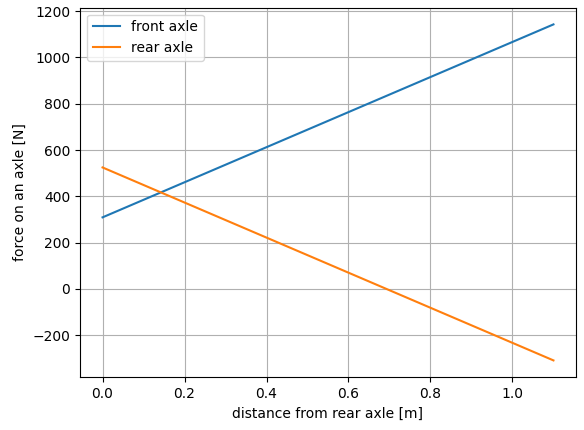
\includegraphics[width=0.5\linewidth]{axles_dynamic_graph}%
\label{fig:dynamic_graph}
\end{figure}

\section{Analytical explanation of safe braking}\label{safe_braking}
\subsection{Maximum potential braking force}\label{safe_braking_max_force}
Braking is limited by the friction between the tires and the surface. Since we stated that in order to brake safely, the rider cannot
skid, we are considering maximum braking force in terms of static friction. As we prooved that the reaction between the bike and 
the surface is always $mg$ in section 2, we can say that the maximum potential braking force is described by equation~\eqref{eq:max_braking_force}. 
\begin{equation}
\centering%
\label{eq:max_braking_force}
F_{\max} = mg\mu
\end{equation}
The $\mu$ in~\eqref{eq:max_braking_force} is static friction coefficient.
\subsection{Keeping rear wheel from lifing off}\label{safe_braking_otb}
\begin{figure}[H]
\caption{}
\centering%
\label{fig:angular_acceleration_figure}
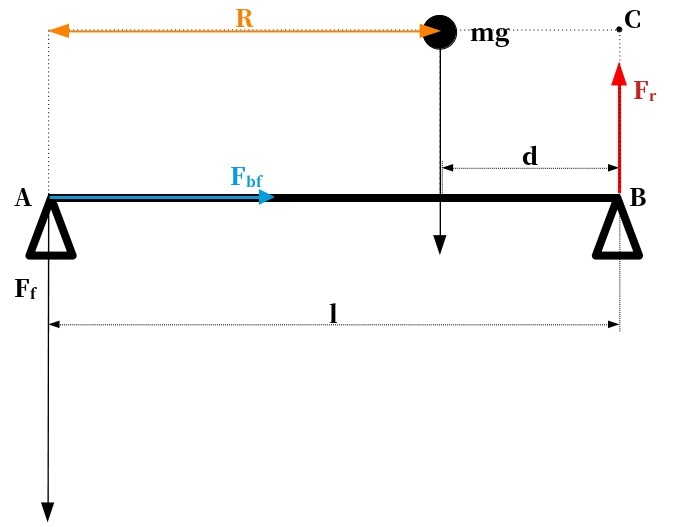
\includegraphics[width=0.5\linewidth]{angular_acceleration_diagram}%
\end{figure}
The most dangerous threat when braking is angular acceleration of the whole bike around the front axle resulting
in rear wheel getting into the air. In order for that to happen, there must be a vector of force pointing upwards
from rear axle, which, as we can see in figure~\ref{fig:dynamic_graph} appears as negative values on the graph.
In order to calculate the angular acceleration ($\alpha$), we need to calculate the moment of inertia of rider 
and bicycle.
\begin{equation}
\centering%
\label{eq:moment_of_inertia}
\sum \tau = F_r \cdot l =  I\alpha = MR^2\alpha
\end{equation}
The sum of torques in our case is the moment excerted by $F_r$ only, as the torque excerted by the $F_f$ is 
zero because we are equating torques to point A (fig.~\ref{fig:angular_acceleration_figure}). Knowing that, $\sum \tau$ can be denoted just as $\tau$. With that, we can
calculate the angular acceleration of the whole body while braking
\begin{equation}
\centering%
\label{eq:angular_acceleration_eq}
\alpha = \frac{\tau}{MR^2}
\end{equation}
\begin{equation}
\centering%
\label{eq:angular_acceleration_fun}
f(d) = \frac{\tau}{M{(l - d)}^2}
\end{equation}
If we plot~\eqref{eq:angular_acceleration_eq} as a function of distance of centre of mass from the rear axle~\eqref{eq:angular_acceleration_fun} 
along with torque and moment of inertia, we can see just how quickly the angular acceleration rises when the centre of mass
gets closer to the axis of rotation. With this graph we can see that when we get close enough to the axis of 
rotation, every centimeter can have a huge impact on the angular acceleration, and in turn the reaction time 
we have to prevent what is widely known as going over the bars.
\begin{figure}[H]
\caption{}
\centering%
\label{fig:angular_acceleration_graph}
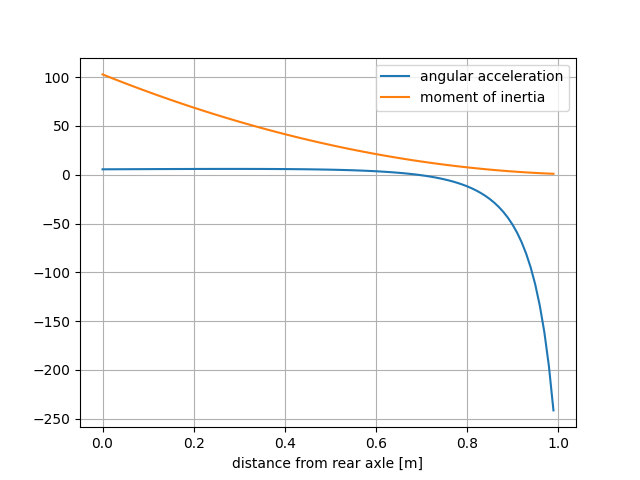
\includegraphics[width=0.8\linewidth]{angular_acceleration}%
\end{figure}
\subsection{Preventing skidding}\label{safe_braking_skidding}
Skidding is another threat while braking, the most dangerous being front wheel skid. In order for skid to happen
the braking force $F_b$ must be higher than the frictional force between ground and the tire $F_f$, so in order 
not to skid the following condition must be met:
\begin{equation}
\centering%
\label{eq:skidding}
F_b < F_f \implies F_b < F_r \cdot \mu
\end{equation}
Having that information, we can put force excerted on either axle in place of $F_r$ and friction coefficient
between the tire and surface as $\mu$ and check for skidding. 
Not skidding also gives us the most effective braking as the static friction coefficient is always higher than 
dynamic one. In case of tire on a pavement, depending on the type of thread, the difference is anywhere from
7\% to 20\%, which is a major change considering that the transition from static to dynamic friction is abrupt,
so the sliding can start unexpectedly.

\section{Combining theoretical model with geometry of a bicycle}\label{geometry}
Geometry of the frame is the most important describing factor of a bicycle. In the beginning of section 2, we
have derived our model of the bicycle, which only describes how long the bike is and how high the centre of the 
mass is in respect to the lever arm, which is between the axles. For further analysis we will use the same model, 
but we will include constraints taken from the geometry of the bicycle. 
\begin{figure}[H]
\caption{}
\centering%
\label{fig:bike_geometry}
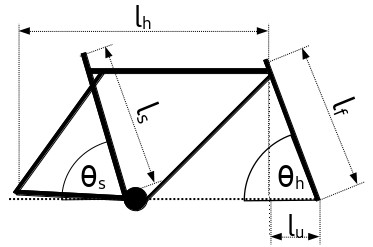
\includegraphics[width=0.5\linewidth]{bike_geometry}%
\end{figure}
\subsection{Finding effective horizontal range of motion}\label{geometry_horizontal_reach}
When it comes to the horizontal range of motion, we only consider how far forward can a rider lean, as it is firmly
determined by the geometry of the bicycle, whereas leaning back is determined more by the height of a rider and because considering 
rider's body in full detail would be too ambiguous and complicated for this analysis, we simply assume that the farthest back the rider can put his centre of mass is over the rear axle.
There are two things that determine the effective range \- the head angle $\theta_h$ (fig.~\ref{fig:bike_geometry}) and the length of the fork $l_f$.
From that, using trigonometric function we can calculate the horizontal effective reach $l_h$~\eqref{eq:effective_reach}.
\begin{equation}
\centering%
\label{eq:effective_reach}
l_h = l - l_f\cos\theta_h
\end{equation}
\subsection{Finding the lowest possible ride height}\label{geometry_lowest_pos}
The other measurement we will consider is the ride-height. First, we will consider the lowest possible ride-height.
This, like the effective horizontal reach, is strictly tied to the geometry of the bicycle. The measurement we will
be interested in is the length of the seattube length $l_s$ (fig.~\ref{fig:bike_geometry}), which is described by the size of frame, and its angle ($\theta_s$).
The minimum height $h_m$ can be calculated by~\eqref{eq:minimum_height}.
\begin{equation}
\centering%
\label{eq:minimum_height}
h_m = l_s\sin\theta_s
\end{equation}
The calculated height would be unachievable in real life, as the body of the rider takes its own form and the centre
of mass will be higher. Because the posture of the rider can take many forms and because making theoretical model 
of human body would be out of scope for this paper, we will simply assume that the centre of mass is 20 
centimeters above the calculated height. %make a measurement
\subsection{Finding optimum height for pedalling}\label{geometry_pedalling_pos}
For finding the optimum pedalling height we will need to consider the lenght of legs of the rider. The rule of thumb 
for finding the optimum saddle height is 90\% of distance between the croutch and the ground. According to that, we 
will find the height on which the centre of mass will be moving just like in case of the lowest point possible, and 
to that we will also add 20 centimeters.

\section{Finding the position for the most effective braking}\label{effective_braking}
Now having developed all necessary analitical tools, we can find the most effective position on a bike for braking. 
We will consider two cases: the lowest possible position and the position optimized for pedalling.
For the bike we will use Biria Pro RS, size 17\"~with the rider's distance from croutch to ground being
90 centimeters [See Appendix B].
\subsection{Finding theoretical maximum}\label{effective_braking_theoretical_max}
First we will consider the absolute theoretical maximum safe braking force with disregard to the grip on the tires or power of the 
brakes. As we have stated in section 3, in order to brake safely, the rider needs to maintain positive angular
acceleration. If we plot a function of braking force from angular acceleration,
\begin{equation}
\centering%
\label{eq:force_from_angular_acceleration}
f(\alpha) = \frac{\alpha mR^2 + mgd - mg}{h}
\end{equation}
\begin{figure}[H]
\caption{}
\centering%
\label{fig:braking_force_graph}
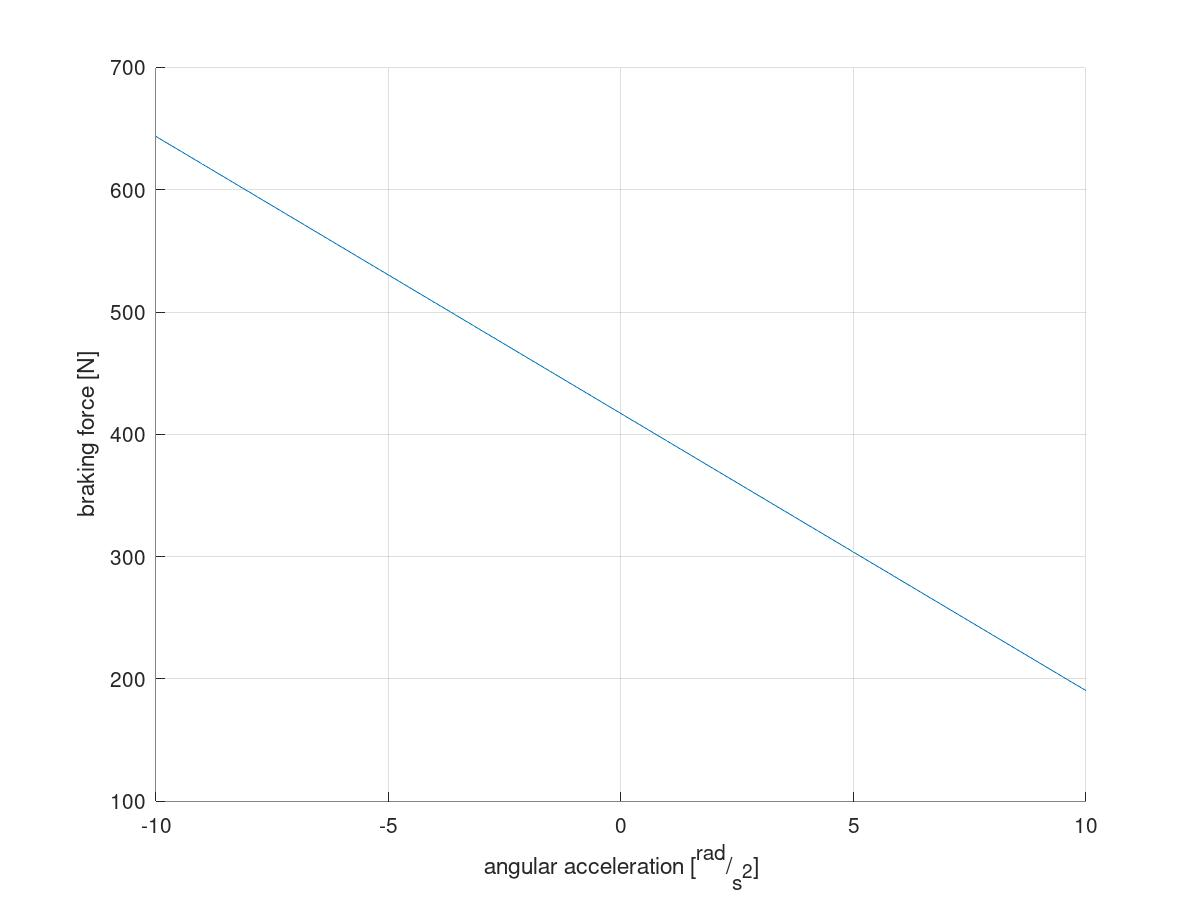
\includegraphics[width=0.7\linewidth]{force_from_angular_acceleration}%
\end{figure}
We can see that the maximum braking force without the rider going over the bars is the value approaching at $0\frac{rad}{s^2}$. It
cannot be zero, as then the force on the rear wheel would be zero, resulting in skidding. Of course, in real world this would not 
make any difference, as the maximum braking force without skidding on rear wheel would also be almost zero, but for the sake of 
finding the theoretical maximum braking force while maintaing safety, the maximum braking force is
\begin{equation}
\centering%
\label{eq:force_from_angular_acceleration}
F_{\max} = \lim_{\alpha\to 0} f(\alpha)
\end{equation}
When we plot these maximum values into a graph we get the following:
\begin{figure}[H]
\caption{}
\centering%
\label{fig:maximum_theoretical_deceleration}
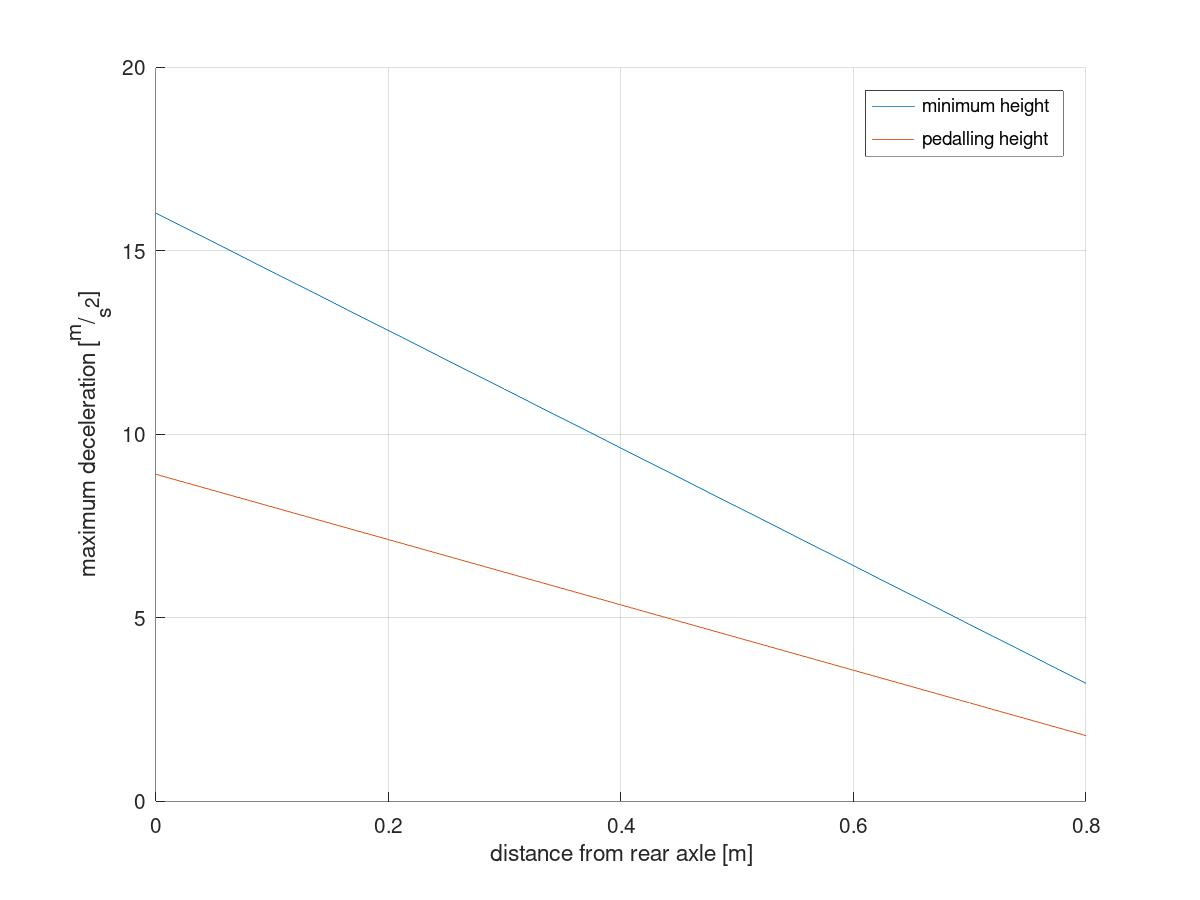
\includegraphics[width=0.7\linewidth]{maximum_theoretical_deceleration}%
\end{figure}
In figure~\ref{fig:maximum_theoretical_deceleration} we can see that the maximum deceleration is the highest nearest the rear axle
which is explained by the fact that the moment of inertia of the system is the highest on the back of the bike making it harder
to lift the rear wheen off the ground. Other thing we can see is the difference in the maximum deceleration between the lowest
position and the pedalling position, this is because the torque excerted on the bike is higher, which has the biggest impact when
the moment of inertia is higher. The values actually converge near the front axle, which means that near the front, the impact 
of the height of the centre of mass is much smaller. 
\subsection{Finding realistic values for braking}\label{effective_braking_realistic_max}
In section~\ref{effective_braking_theoretical_max} we calculated theoretical maximum braking force while maintaining
rules for safe braking outlined in section~\ref{theory_rules}. 
In section~\ref{safe_braking_max_force} we found that the maximum braking force is $mg\mu$, which will be the absolute
maximum braking force, however, we will not be able to maintain this value across the whole range of motion as 
either skidding or going over the bars would occur, so  this is where the theoretical maximum comes into play. 
When the theoretical maximum falls below the practical maximum force ($mg\mu$), it is possible to brake with such force, 
as the condition for not skidding from section~\ref{safe_braking_skidding} is met. 
\begin{figure}[H]
\caption{}
\centering%
\label{fig:maximum_practical_deceleration}
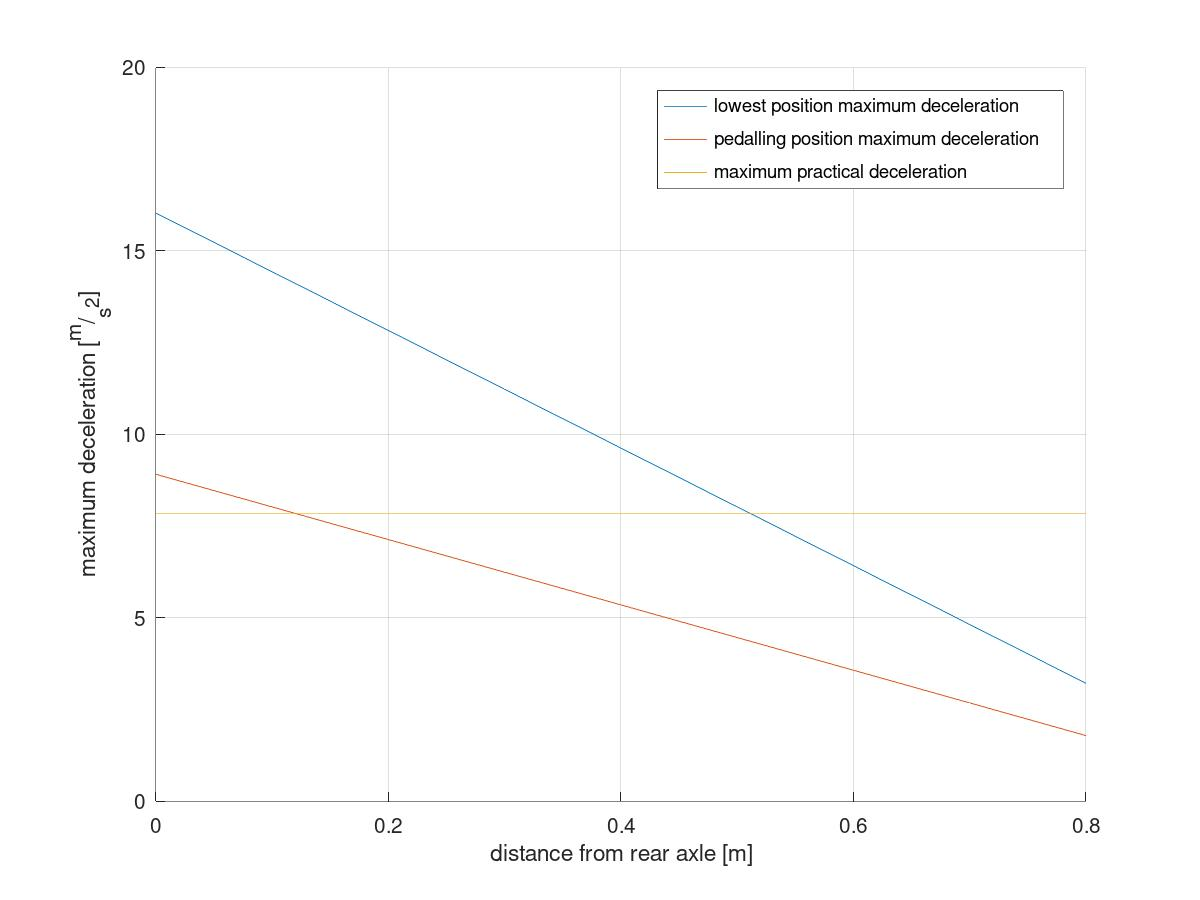
\includegraphics[width=0.7\linewidth]{maximum_practical_deceleration}%
\end{figure}
When looking at the combined plot of practical and theoretical maximum braking force (fig.~\ref{fig:maximum_practical_deceleration}), 
the realistic deceleration is the lowest possible value and with that we can see that for low-seat position the cyclist can brake 
with maximum force up until $0.5m$ from rear axle, whereas when in high position, only until $0.15m$. We can now see that the 
position of centre of mass for maximum braking power is not a point but rather a range of motion whose length is dependent on 
the following factors: grip of the tires, height of the seat, length of the bike and the mass of the rider. 
In section~\ref{effective_braking_factors}
\subsection{Other factors impacting braking}\label{effective_braking_factors}
In order to visualize the impact of different factors on effectiveness of braking, we will take the same arguments we used across the 
whole analysis [See Appendix A] and change one variable to see how it will impact the maximum braking range.
\subsubsection{Friction coefficient between tires and ground}
\begin{figure}[H]
\begin{minipage}[t]{.6\linewidth}
\vspace{0pt}
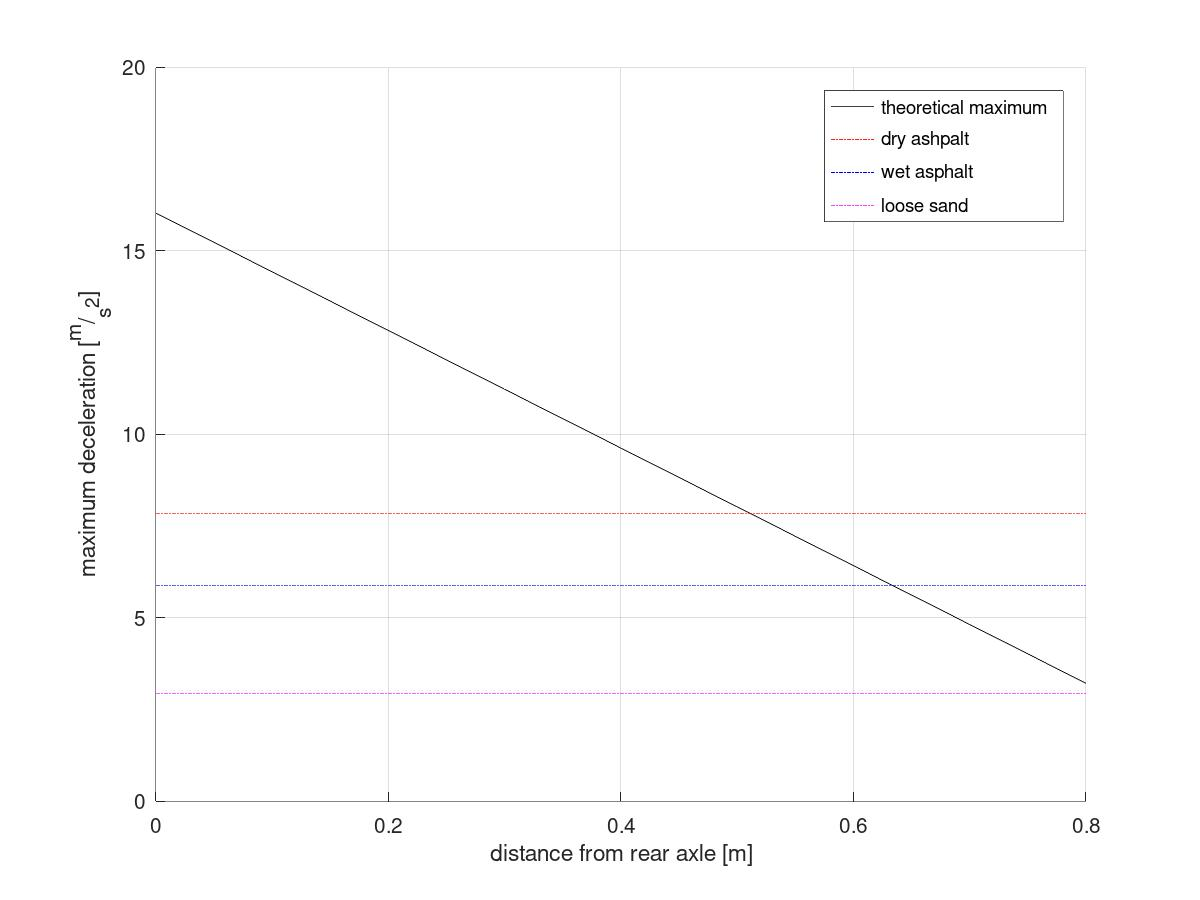
\includegraphics[width = \linewidth]{friction_on_braking}
\end{minipage}%
\begin{minipage}[t]{0.4\linewidth}
\vspace{0pt}
\centering
\begin{tabular}{|c | c | c | c|} 
\hline
surface & $\mu$ & $a_{\max} [\frac{m}{s^2}]$ & $d_{\max}[m]$ \\ [0.5ex] 
\hline\hline
dry asphalt & 0.8 & 7.84 & 0.52 \\ [1ex] 
wet ashpalt & 0.6 & 5.88 & 0.63 \\ [1ex]
loose sand & 0.3 & 2.94 & 0.82 \\ [1ex]
\hline
\end{tabular}
\end{minipage}%
\caption{}%
\label{friction_on_braking}
\end{figure}
We can see that with the increase of $\mu$ the maximum braking range $d_{\max}$ gets shorter, but the maximum deceleration $a_{\max}$ 
increases. (Wilson 2004, 246)
\subsubsection{Seat height}
\begin{figure}[H]
\begin{minipage}[t]{.6\linewidth}
\vspace{0pt}
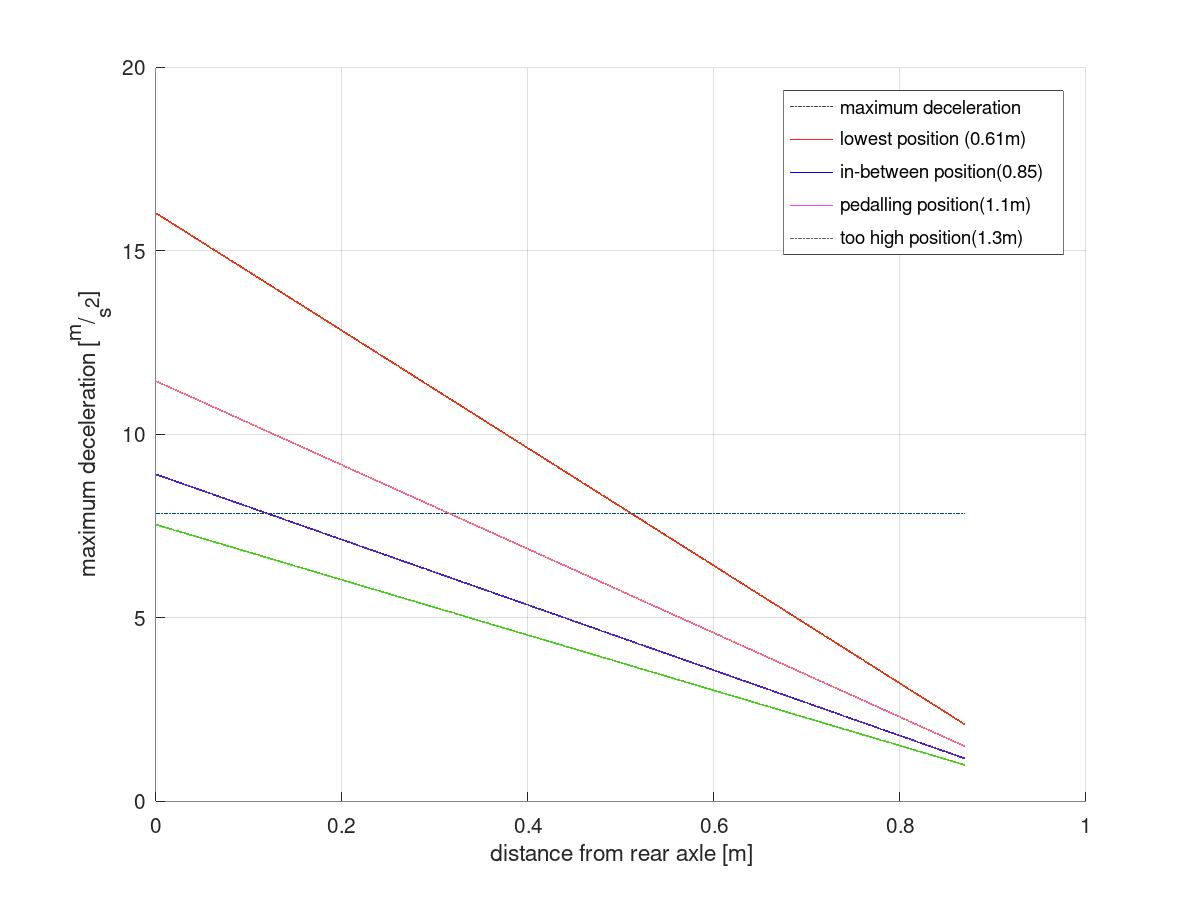
\includegraphics[width = \linewidth]{height_on_braking}
\end{minipage}%
\begin{minipage}[t]{0.4\linewidth}
\vspace{0pt}
\centering
\begin{tabular}{|c | c | c|} 
\hline
 h$[m]$ & $a_{\max} [\frac{m}{s^2}]$ & $d_{\max}[m]$ \\ [0.5ex] 
\hline\hline
0.61 & 7.84 & 0.52 \\ [1ex] 
0.85 & 7.84 & 0.32 \\ [1ex]
1.1 & 7.84 & 0.12 \\ [1ex]
1.3 & 7.53 & 0 \\ [1ex]
\hline
\end{tabular}
\end{minipage}%
\caption{}%
\label{friction_on_braking}
\end{figure}
We can see that the maximum deceleration stays the same, what changes is the range of maximum braking $d_{\max}$, the lower the 
centre of mass, the longer it is. The relation between the height and the maximum active braking force is rational, as height is 
in the denominator~\eqref{eq:force_from_angular_acceleration}, so the same difference higher up has less impact than the same one lower.
\subsubsection{Mass}
\begin{figure}[H]
\begin{minipage}[t]{.6\linewidth}
\vspace{0pt}
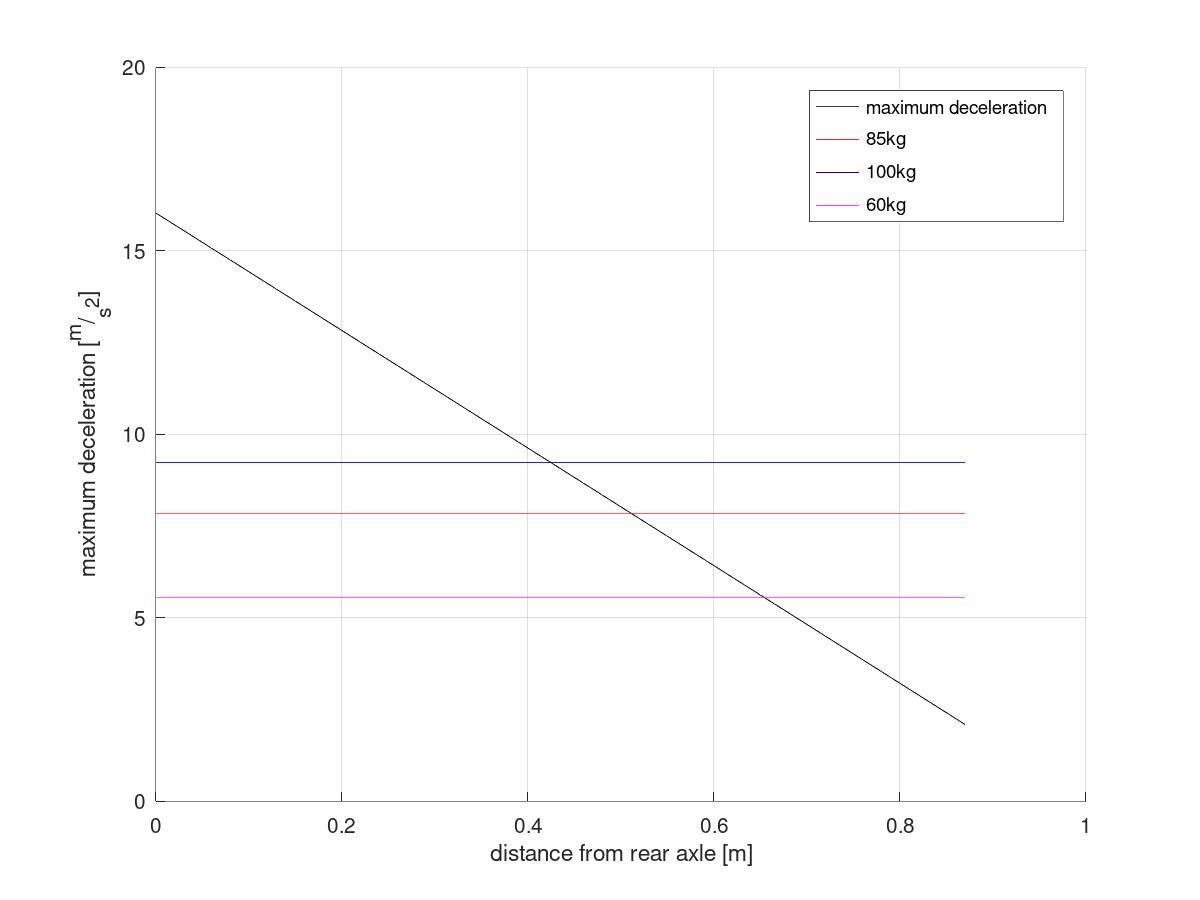
\includegraphics[width = \linewidth]{mass_on_braking}
\end{minipage}%
\begin{minipage}[t]{0.4\linewidth}
\vspace{0pt}
\centering
\begin{tabular}{|c | c | c|} 
\hline
 m$[kg]$ & $a_{\max} [\frac{m}{s^2}]$ & $d_{\max}[m]$ \\ [0.5ex] 
\hline\hline
60 & 5.54  & 0.52 \\ [1ex] 
85 & 7.84 & 0.32 \\ [1ex]
100 & 9.23 & 0.2 \\ [1ex]
\hline
\end{tabular}
\end{minipage}%
\caption{}%
\label{mass_on_braking}
\end{figure}
We can see that the mass has the same effect as friction coefficient on braking. What may seem perplexing is that the 
heavier the rider would decelerate faster than a lighter one. This is true to our analysis, because we are talking about the 
maximum and such rider would brake faster on sufficient brakes than a lighter one. Of course, in real world, we would encounter
many more roadblocks in achieving the maximum for heavier rider because the brakes would have to be very powerful and 
thermo-efficient. So the mass of the rider determines the power of the brakes regardless of the friction coefficient.

\section{Real-life applications}\label{applications}
Knowing the heart of the problem of braking on a bicycle, we can now consider applications in real life to the analysis derived above.
\subsection{Emergency braking}
As stated in the introduction, tutorials on techniques on bicycle are very vague in detail and revolving around the experience of the 
presenter. This analysis can fill in the holes with objective facts. The tips derived from our analysis would be the following:
\begin{itemize}
\item{Your position on the bike determines the braking effectiveness than your brakes~-~when you want to stop fast, keep your centre
of mass farther back}
\item{The range at which you can brake at the biggest rate is determined by the height of your centre of mass, the lower your seat, the
farther up the bike front you can use your brakes confidently}
\item{The farther back your centre of mass is the more evenly you can split braking force between front and rear, minimizing losses in braking power
due to heat and pad residue}
\item{Pay attention to your tires, friction between the tire and the surface has bigger impact on braking performance than brakes themselves}
\item{Don't use full braking power unless you are on consistent surface, changes in friction will cause you to either skid or go over
the bars}
\item{When on loose or wet surface, use less force on the brakes and move slightly more forward to prevent accidental front-wheel skidding}
\end{itemize}
\subsection{Bike-fitting}
Finding the right size of bike is essential for safety of the rider. Aside from a handful of imcompatibilities between the rider and the
bike, one is the most important: size. When the bike is too small, it will cause the rider's centre of mass to be closer to the front
of the bike making his moment of inertia low, which makes him vulnerable to going over the bars. Too big bike on the other hand might
cause front wheel skid, which is just as dangerous as going over the bars. This is caused by too little load on the front wheel, which 
combined with strong enough brake, might break the grip more easilly.
\subsection{Choosing parts}
When buying parts, it is very important not to cheap out on parts that are essential for rider's safety. When it comes to braking, these
are brakes and tires. \textbf{Brakes} should be strong enough to decelerate the rider at the highest possible rate, because the
maximum braking force is expressed by $F_b = mg\mu$, the biggest factor to be taken into consideration is the weight of the rider, so
the heavier the rider the more heavy-duty the brakes should be. Other factor is modulation of the brake, i.e.~how precise the brake
is. When in the range of maximum braking, the biggest deceleration is achieved by applying maximum braking force on both brakes 
seperately, so the more precise the brake, the further the rider can push the brakes. The two most popular brake types are rim and
disk brakes. The risk with the rim brake is that it can be easilly contaminated which can cause changes in friction between pads and
the rim. Disk brakes do not have that problem, but they can overheat more easilly whose effect is more gradule than sudden contamination
or even rim getting wet, so disk brakes are more reliable option. \textbf{Tires} are just as important, where brakes provide the actual
braking, the tires give the potential for effective braking, as mentioned before, maximum braking is determined by mass and friction
coefficient. This coefficient changes in relation to surface, but at least a tire in good condition will maximize this coefficient
and ensure consistent friction across the whole surface of the tire. 
\subsection{Unambigous tool for analysing athletes' performance}
Using such model combined with sensory data would enable to quantify the technique of a rider. Knowing how effective a cyclist
in using his brakes would give a good insight to better safety and performance.

\section{Issues with the analysis}
This analysis both shows why the existing sources of knowledge are not specific enough and why it is the best way to approach teaching
people about this problem.
\subsection{Expressing the problem in centre of the mass only}
In order to make this analysis, it was necessary to simplify the system as much as possible in order to get rid of as many ambiguities
as possible. One of such ambiguities is body of the rider. When riding a cyclist can take many positions resulting in the same centre
of mass, which in turn makes the analysis too complex. The problem with this approach is that centre of mass is not intuitive. As the
rider leans more and more backwards, his body folds, which causes his centre of mass to be farther away from his actual body. This 
means that the more leaned back the rider is, the less of an impact his movement has in relation to the centre of mass. On the other
hand the more leaned forward the cyclist is, the more straight his posture is, which means that his movement has a lot bigger impact 
on the position of his centre of mass. The more complex and intuitive way to present this problem would be to take the point of 
reference to the pelvis of the rider and map his position onto the bike and calculate the centre of mass from frame to frame resulting
in more intuitive representation.
\subsection{No easy way to confirm the theoretical in an unambigous experiment}
A big issue is measuring braking force on a real bicycle. Measuring and recording braking force in real time is a big problem when 
mobile. In order to measure this force, we would need to know the friction coefficient between the braking surface and the pad along
with data how it changes due to heat. Other thing is the inner workings of a specific brake which would give us the information about
how the force on the lever translates onto the brake. Lastly we would need enough bravery to actually reach the edge values, which
is risky because the tester would have to defy his own instincts in many cases. Such experiment would be possible but it would be risky
and the results would contain a big measurement error from the experimenter alone.

\section{Conclusion}
It is possible to derive an objective physical analysis of braking on the bicycle. As stated in section 7, this is not a perfect model, 
it is based on ideal conditions and gives theoretical maxima, its purpose is to educate on 
what impact does a proper technique, fit, and parts have on the safety. Even though this is only a simple model, it should be sufficient
to give a base to a new person to cycling of how things work without crashing and more importantly a set of objective facts that will
enable for recognizing dangerous tips from tutorials that are given by inexperienced riders.

\section{Appendices}
\subsection{Appendix A}
Links to sample tutorials:
\begin{enumerate}
\item Global Cycling Network ``How to brake like a pro~- Road Cycling'' Global Cycling Network, September 11, 2013, YouTube video, 3:02, \url{https://www.youtube.com/watch?v=frIKK_XU-qE&t=1s}
\item Global Mountain Bike Network ``How To Use Your Brakes Like A Pro Mountain Biker | MTB Breaking Tips'' Global Mountain Bike Network, February 12, 2020, YouTube video, 5:42, \url{https://www.youtube.com/watch?v=0mS7Ga3c5Rc}
\end{enumerate}
\section{Bibliography}
\begin{enumerate}
\item{Wilson, David G. ``Braking'' In \textit{Bicycling Science}, 236~-261, Cambridge, Mass.: MIT Press}
%engineering textbook
%undergrad textbook
\item Global Cycling Network ``How to brake like a pro~- Road Cycling'' Global Cycling Network, September 11, 2013, YouTube video, 3:02, \url{https://www.youtube.com/watch?v=frIKK_XU-qE&t=1s}
\item Global Mountain Bike Network ``How To Use Your Brakes Like A Pro Mountain Biker | MTB Breaking Tips'' Global Mountain Bike Network, February 12, 2020, YouTube video, 5:42, \url{https://www.youtube.com/watch?v=0mS7Ga3c5Rc}
\end{enumerate}
\end{document}
